\documentclass[11pt,a4paper]{article}
\usepackage[latin1]{inputenc}
\usepackage[english]{babel}
% some standard packages
\usepackage{textcomp}
\usepackage{gensymb}
\usepackage{tabularx}
\usepackage{setspace}
\usepackage{xspace}
\usepackage{verbatim}
\usepackage{graphicx}
\usepackage{caption}
\usepackage{subcaption}
\usepackage{url} 
\usepackage{tikz}
\usetikzlibrary{shapes,positioning}

\usepackage{owl}
% begin / end environments
\usepackage{amssymb,amsmath}

\usepackage{amsthm}
\newtheorem{examp}{Example}



\author{Samantha Bail}
\begin{document}

\begin{examp}
\begin{alignat*}{2}
		\K = \{&\ax{Cat \sqsubseteq Carnivore} & \quad\quad &\ax{Carnivore \sqsubseteq Animal \conj \forall eats.Animal}\\
		&\ax{Plant \sqsubseteq \lnot Animal} & \quad\quad & \ax{PetOwner \equiv Human\conj \exists hasPet.Animal}\\
		& \ax{Grass \sqsubseteq Plant} &&\\
		&\ax{Cat(Molly)} & \quad\quad &\ax{hasPet(Alice, Molly)}\\
		&\ax{Human(Alice)} \}\label{ex:petkb}
	\end{alignat*}
\end{examp}

\begin{examp}
\begin{alignat*}{2}
		\K' = \{&\ax{Cat \sqsubseteq Carnivore} & \quad\quad &\ax{Carnivore \sqsubseteq Animal \conj \forall eats.Animal}\\
		&\ax{Plant \sqsubseteq \lnot Animal} & \quad\quad & \ax{PetOwner \equiv Human\conj \exists hasPet.Animal} \\
    	&\ax{Grass \sqsubseteq Plant} & \quad\quad &  \ax{SickCat \equiv Cat \conj \exists eats.Grass} \\
		&\ax{Cat(Molly)} & \quad\quad &\ax{hasPet(Alice, Molly)}\\
		&\ax{Human(Alice)} \}
	\end{alignat*}
\end{examp}


\begin{examp}
\begin{alignat*}{2}
 (\alpha_{1})  & \quad\quad & &\dlax{A \subcls \exists r.A}  \\
 (\alpha_{2})  & \quad\quad & &\dlax{A \subcls Y}  \\	
 (\alpha_{2})  & \quad\quad & &\dlax{\exists r.Y \subcls  B}  \\
 (\alpha_{4})  & \quad\quad & &\dlax{Y \subcls B}   \\
\end{alignat*}
\end{examp}

\begin{table}[h!]
\footnotesize
\begin{tabular}{rlrl}
		(1)&\ax{Cat \sqsubseteq Carnivore}												&(4)&\ax{Grass \sqsubseteq Plant}\\
		(2)&\ax{Carnivore \sqsubseteq Animal \conj \forall eats.Animal}	&(5)&\ax{PetOwner \equiv Human\conj \exists hasPet.Animal}\\
		(3)&\ax{Plant \sqsubseteq \lnot Animal}											&(6)&\ax{SickCat \equiv Cat \conj \exists eats.Grass}
\end{tabular}
\end{table}


\begin{examp}
\begin{alignat}{2}
		\ax{Cat \sqsubseteq Carnivore}	& \quad\quad & &	\ax{Grass \sqsubseteq Plant}\\
		\ax{Carnivore \sqsubseteq Animal \conj \forall eats.Animal} & \quad\quad & & \ax{PetOwner \equiv Human\conj \exists hasPet.Animal}\\
		\ax{Plant \sqsubseteq \lnot Animal}	& \quad\quad & & \ax{SickCat \equiv Cat \conj \exists eats.Grass}
	\end{alignat}
\end{examp}



\begin{examp}
~\newline ~\newline
\begin{tabular}{rlrl}
		(1)&\ax{Cat \sqsubseteq Carnivore}												&(4)&\ax{Grass \sqsubseteq Plant}\\
		(2)&\ax{Carnivore \sqsubseteq Animal \conj \forall eats.Animal}	&(5)&\ax{PetOwner \equiv Human\conj \exists hasPet.Animal}\\
		(3)&\ax{Plant \sqsubseteq \lnot Animal}											&(6)&\ax{SickCat \equiv Cat \conj \exists eats.Grass}
\end{tabular}
\end{examp}



\begin{figure}
\centering{
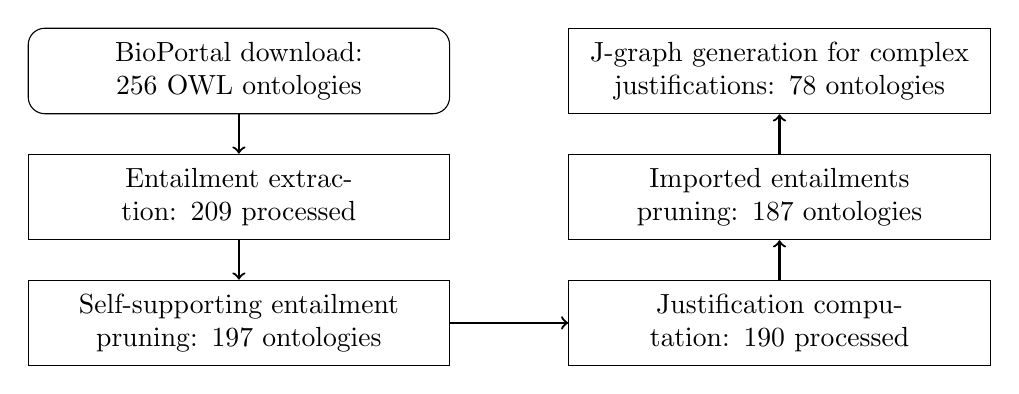
\begin{tikzpicture}
\tikzstyle{every node}=[draw, inner sep=5pt, node distance = 1.3cm, text width=5cm, text centered];

\node[rounded corners=6pt] (download) {BioPortal download: 256 OWL ontologies};
\node[below = 0.5cm of download] (a) {Entailment extraction: 209 processed};
\node [below = 0.5cm of a] (b) {Self-supporting entailment pruning: 197 ontologies};
\node [right = 1.5cm of b] (c) {Justification computation: 190 processed};
\node [above = 0.5cm of c] (d) {Imported entailments pruning: 187 ontologies};
\node [above = 0.5cm of d] (e) {J-graph generation for complex justifications: 78 ontologies};

\foreach \from/\to in {download/a, a/b, b/c, c/d, d/e}
\draw [->,thick] (\from) -- (\to);

\end{tikzpicture}


\caption{A decision tree for categorising entailments.}
\label{fig:entailmenthierarchy}
}
\end{figure}
\newpage


\begin{figure}
\centering{
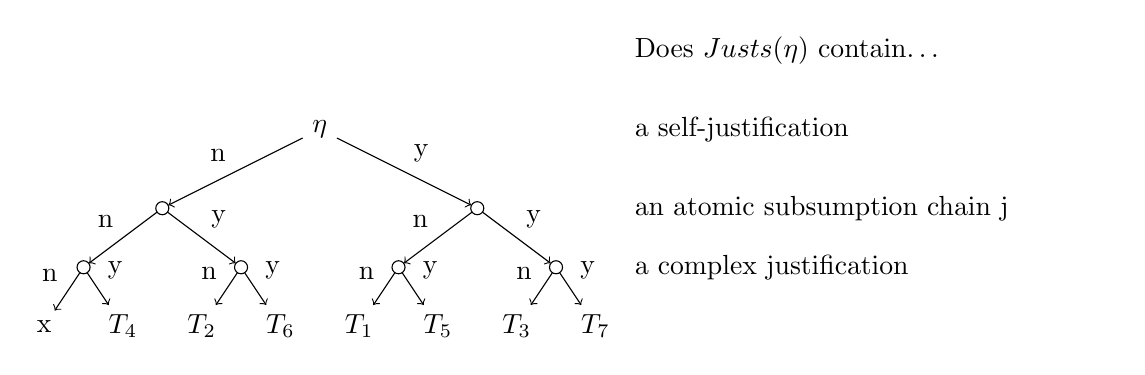
\begin{tikzpicture}[scale=1,->,auto=left]
  
%  \draw (-2,8.25) -- (6,8.25) -- (6,7.75) -- (-2,7.75) -- cycle;
% \draw (-2,7.5) -- (6,7.5) -- (6,7) -- (-2,7) -- cycle;
%  \draw (-2,8.25) -- (6,8.25) -- (6,7.75) -- (-2,7.75) -- cycle;
\node[align=left,text width=6cm] at (9,10) {Does $Justs(\eta)$ contain\ldots};
\node[align=left,text width=6cm] at (9,9) {a self-justification};
\node[align=left,text width=6cm] at (9,8) {an atomic subsumption chain j};
\node[align=left,text width=6cm] at (9,7.25) {a complex justification};
  
\node[draw=none] (root) at (2,9) {$\eta$};

\tikzstyle{every node} = [color=black,shape=circle,scale=0.5,draw]
  
\node (n) at (0,8)  {};
\node (y) at (4,8)  {};
\node (nn) at (-1,7.25)  {};
\node (ny) at (1,7.25)  {};
\node (yn) at (3,7.25)  {};
\node (yy) at (5,7.25)  {};

\tikzstyle{every node} = [draw=none]
\node[draw=none] (nnn) at (-1.5,6.5)  {x};

\node (nny) at (-0.5,6.5)  {$T_{4}$};	
\node (nyn) at (0.5,6.5)  {$T_{2}$};
\node (nyy) at (1.5,6.5)  {$T_{6}$};
\node (ynn) at (2.5,6.5)  {$T_{1}$};
\node (yny) at (3.5,6.5)  {$T_{5}$};
\node (yyn) at (4.5,6.5)  {$T_{3}$};
\node (yyy) at (5.5,6.5)  {$T_{7}$};



\draw (root) to node [swap]  {n} (n);
\draw (root) to node {y} (y);

\draw (n) to node [swap] {n} (nn);
\draw (n) to node {y} (ny);

\draw (nn) to node [swap]  {n} (nnn);
\draw (nn) to node {y} (nny);

\draw (ny) to node [swap]  {n} (nyn);
\draw (ny) to node {y} (nyy);

\draw (y) to node [swap]  {n} (yn);
\draw (y) to node {y} (yy);

\draw (yn) to node  [swap] {n} (ynn);
\draw (yn) to node  {y} (yny);

\draw (yy) to node [swap]  {n} (yyn);
\draw (yy) to node  {y} (yyy);


\end{tikzpicture}
\caption{A decision tree for categorising entailments.}
\label{fig:entailmenthierarchy}
}
\end{figure}
\newpage

\begin{figure}
\centering
		\begin{subfigure}{0.4\textwidth}
                \centering
                \input{../img/asserted-cg.tex}
                \caption{Asserted class graph.}
        	\label{fig:asserted}
        \end{subfigure}%
        ~ %add desired spacing between images, e. g. ~, \quad, \qquad etc. 
          %(or a blank line to force the subfigure onto a new line)
		\begin{subfigure}{0.6\textwidth}
                \centering
                \input{../img/inferred-cg.tex}
                \caption{Inferred class graph.}
        	\label{fig:inferred}
        \end{subfigure}
\end{figure}


Lorem ipsum dolor sit amet, consectetur adipiscing elit. Sed pulvinar erat at mi facilisis condimentum. Sed bibendum arcu nec erat venenatis nec venenatis enim pulvinar. Fusce nunc dolor, mollis sit amet faucibus ac, accumsan id odio. In enim ligula, placerat pharetra commodo non, pulvinar at libero. Vestibulum nisi leo, consequat ut accumsan nec, pellentesque ac elit. Aliquam at facilisis sapien. Nunc sed velit et enim elementum commodo mattis ac eros. Aliquam libero sapien, eleifend vitae consequat eget, dictum a lorem. Mauris feugiat ligula non tortor feugiat eget malesuada purus ultrices. Praesent viverra tristique orci nec dapibus. Cras at augue eget est ultricies auctor. Sed condimentum dolor sed ipsum bibendum eget placerat nisi ultrices. Duis et condimentum tellus. Duis mi urna, pulvinar vitae scelerisque non, vestibulum sed massa. Vestibulum cursus, enim sit amet tincidunt posuere, nunc lectus aliquam quam, in malesuada turpis odio quis elit. Curabitur in tincidunt velit.


\end{document}